\documentclass[12pt]{article}
\usepackage[T1]{fontenc}
\usepackage[T1]{polski}
\newcommand{\BibTeX}{{\sc Bib}\TeX}
\usepackage{graphicx}
\usepackage{hyperref}
\usepackage{amsmath} \usepackage{amssymb} \usepackage{amsfonts}
\usepackage[utf8]{inputenc}
\usepackage{minted}
\newcommand{\cljt}[1]{\mintinline{clojure}{#1}}
\usepackage{tikz-cd}
\setlength{\textheight}{21cm}

\title{{\bf Zadanie nr 2 - Próbkowanie i Kwantyzacja}\linebreak
	Cyfrowe Przetwarzanie Sygnałów}
\author{Jakub Mileczarek 236602 \and Antoni Jończyk, 236551}
\date{2023-03-13} % jak zdążymy xd

\begin{document}
\clearpage\maketitle
\thispagestyle{empty}
\newpage
\setcounter{page}{1}
\section{Cel zadania}
Celem zadania było zaimplementowanie konwersji analogowo-cyfrowej i
cyfrowo-analogowej.\cite{instrukcja2}
\section{na razie sam pokaz}
\subsection{próbkowanie}
\begin{figure}[H]
	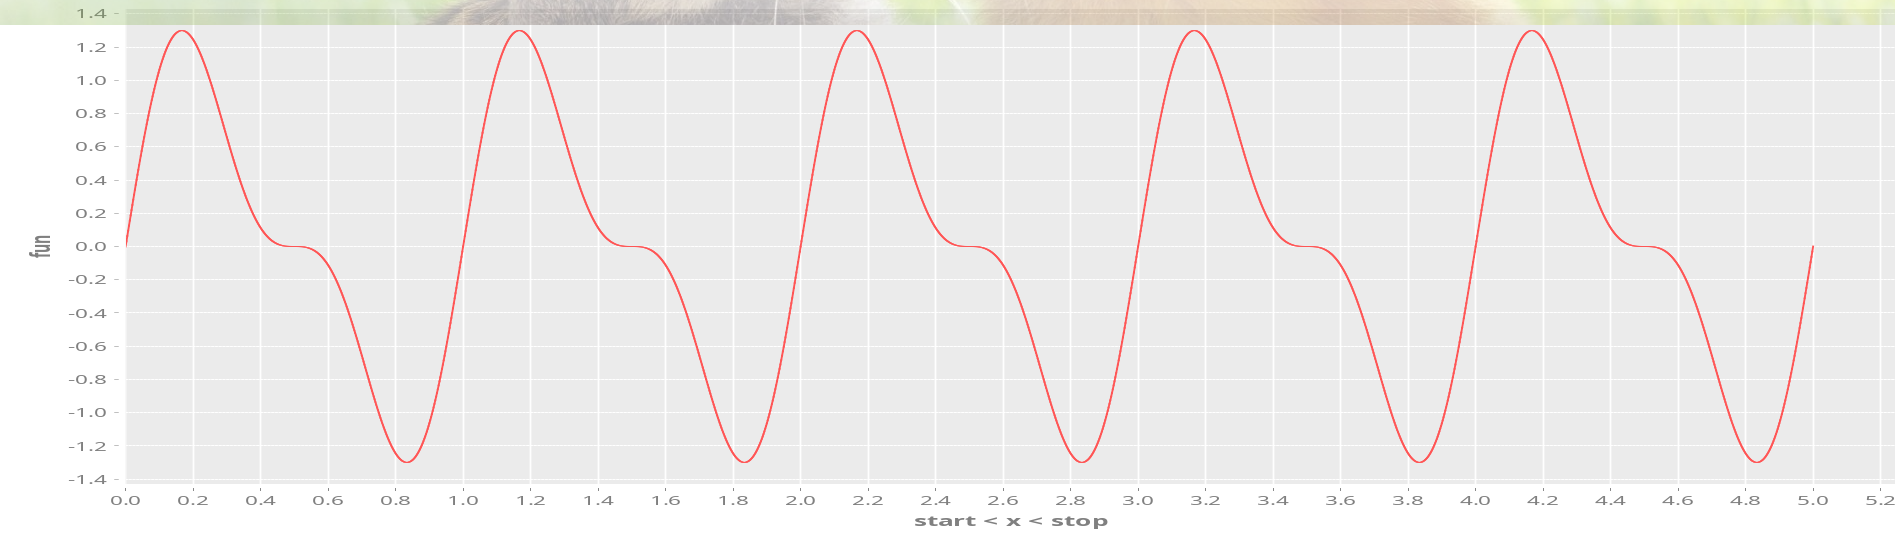
\includegraphics[width=\linewidth]{2a.png}
	\caption{funkcja $\sin x +\frac{\sin 2x}{2}$}
\end{figure}

\begin{figure}[H]
	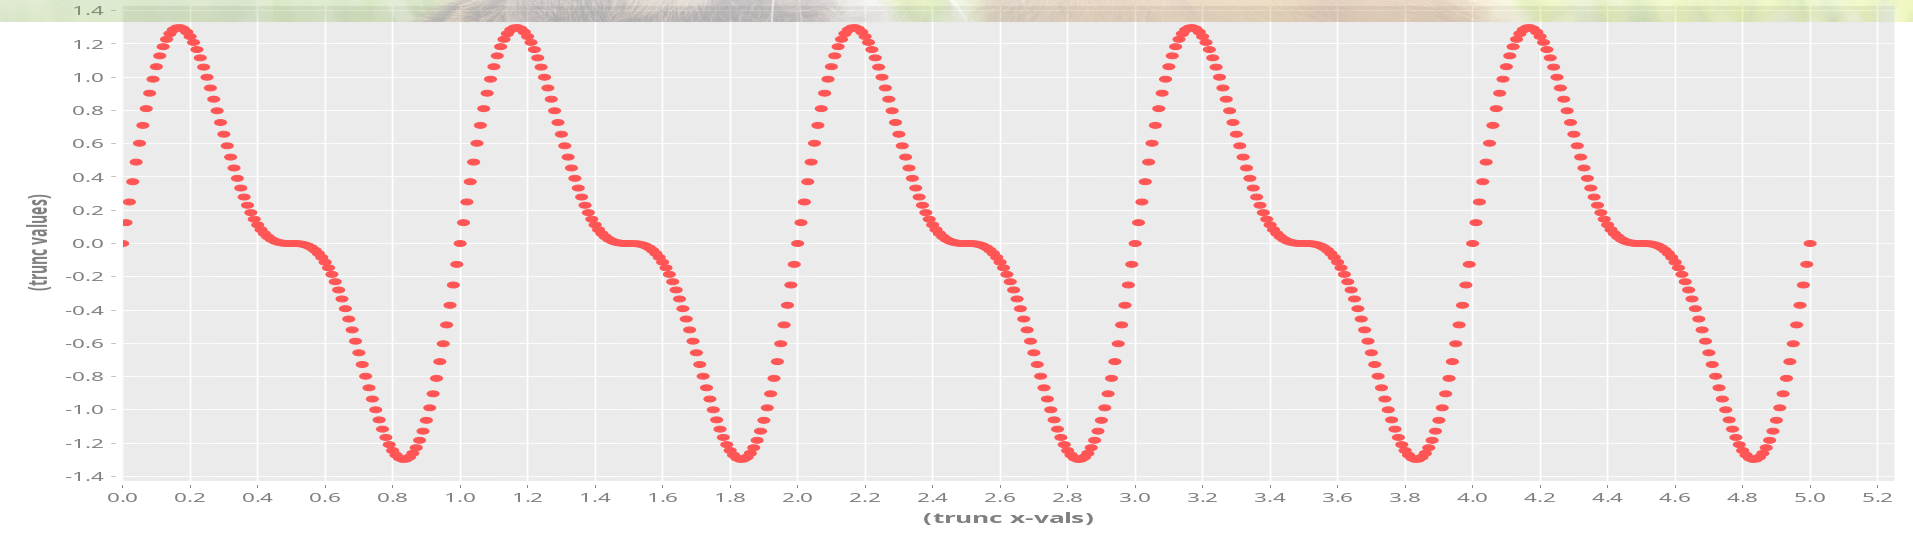
\includegraphics[width=\linewidth]{2a100.png}
	\caption{funkcja spróbkowana z częstotliwością 100Hz}
\end{figure}

\begin{figure}[H]
	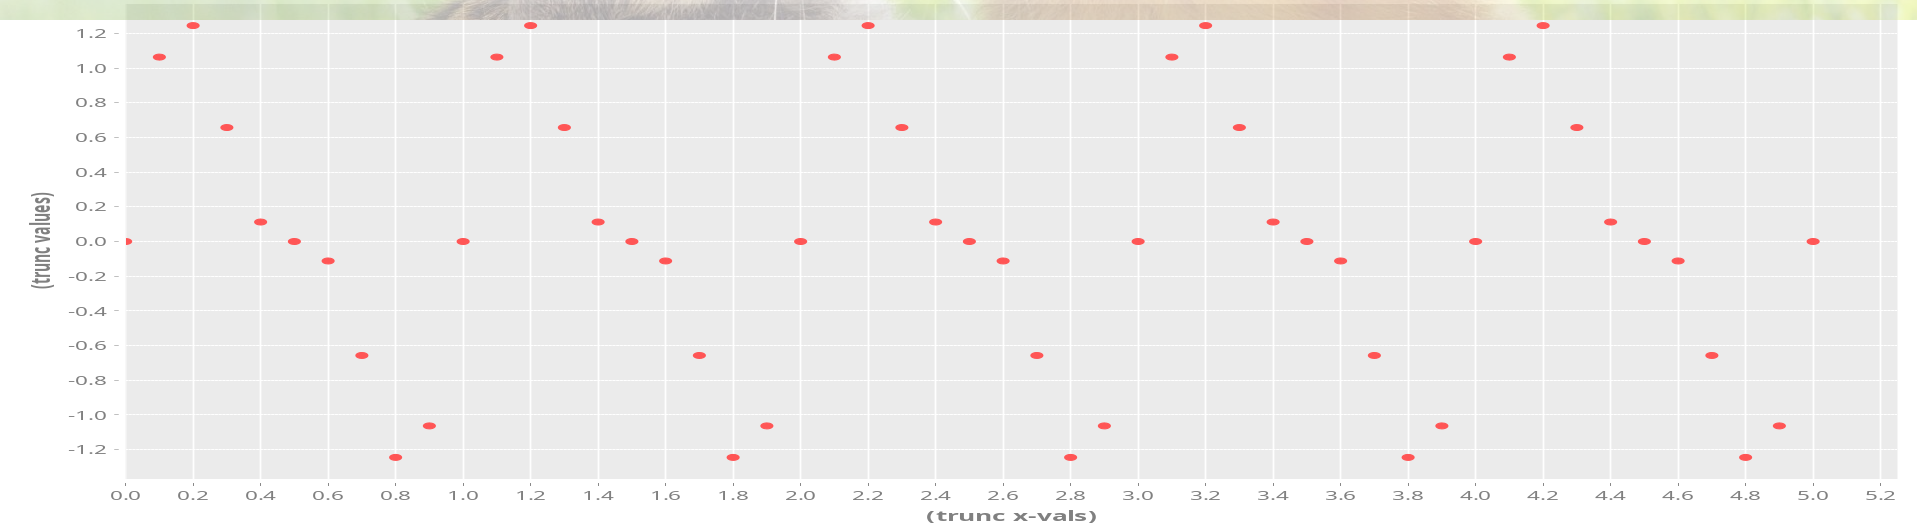
\includegraphics[width=\linewidth]{2a10.png}
	\caption{funkcja spróbkowana z częstotliwością 10Hz}
	\label{only}
\end{figure}

\subsection{kwantyzacja}
zastosowaliśmy kwantyzację z zaokrąglaniem


\begin{figure}[H]
	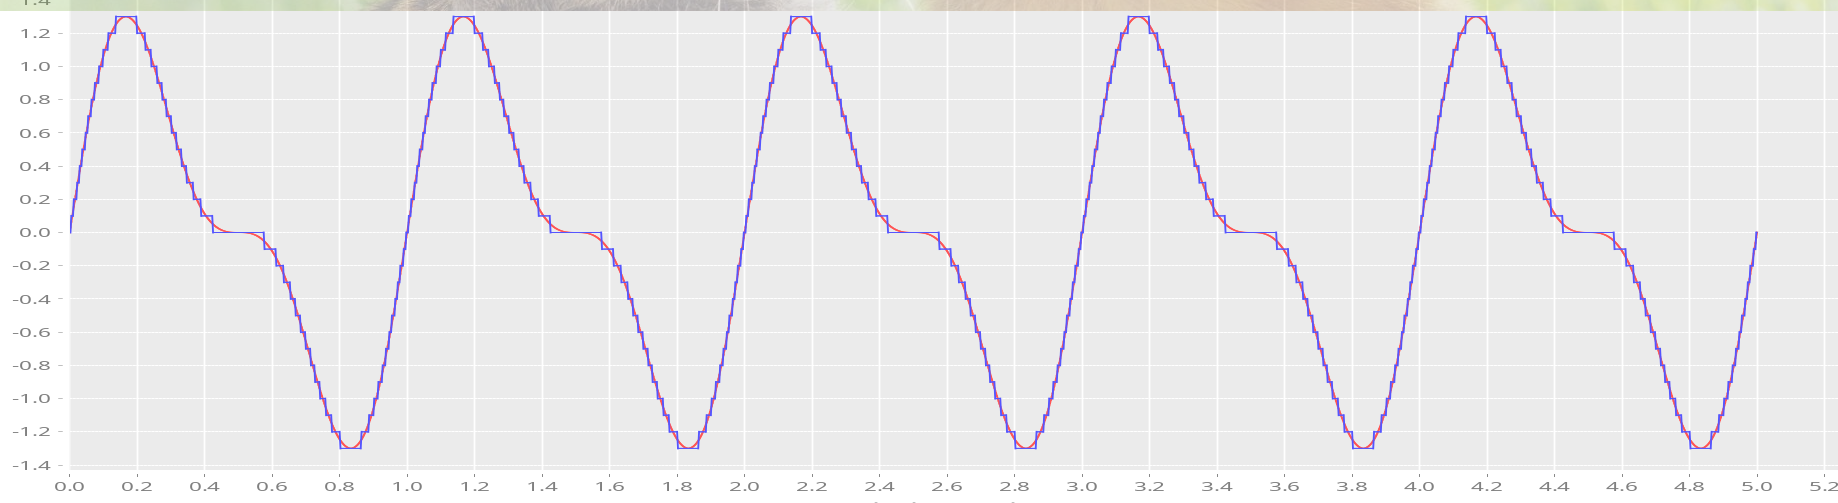
\includegraphics[width=\linewidth]{2akwant01.png}
	\caption{kwantyzacja z krokiem równym $0.1$}
\end{figure}


\begin{figure}[H]
	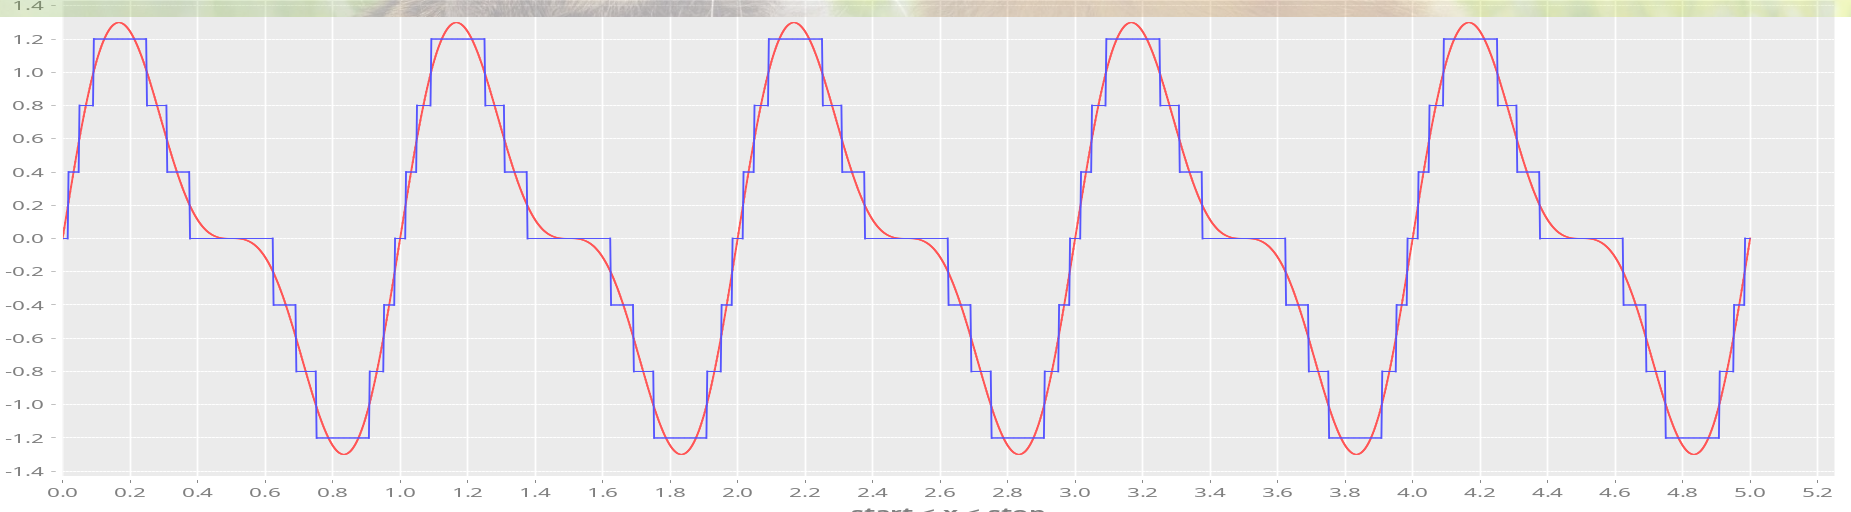
\includegraphics[width=\linewidth]{2akwant04.png}
	\caption{kwantyzacja z krokiem równym $0.4$}
\end{figure}

\begin{figure}[H]
	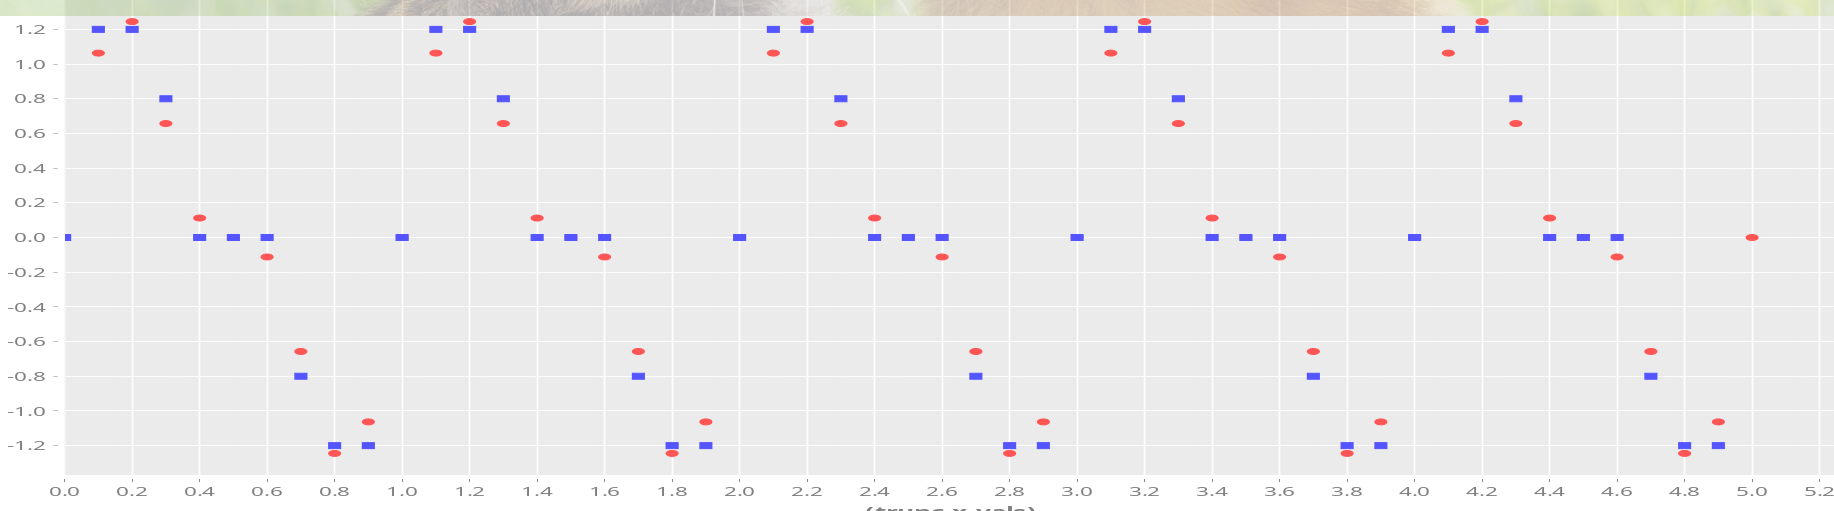
\includegraphics[width=\linewidth]{2aboth.png}
	\caption{kwantyzacja z krokiem równym $0.4$ i dyskretyzacja z częstotliwością 10Hz}
	\label{both}
\end{figure}


\subsection{interpolacja}

\begin{figure}[H]
	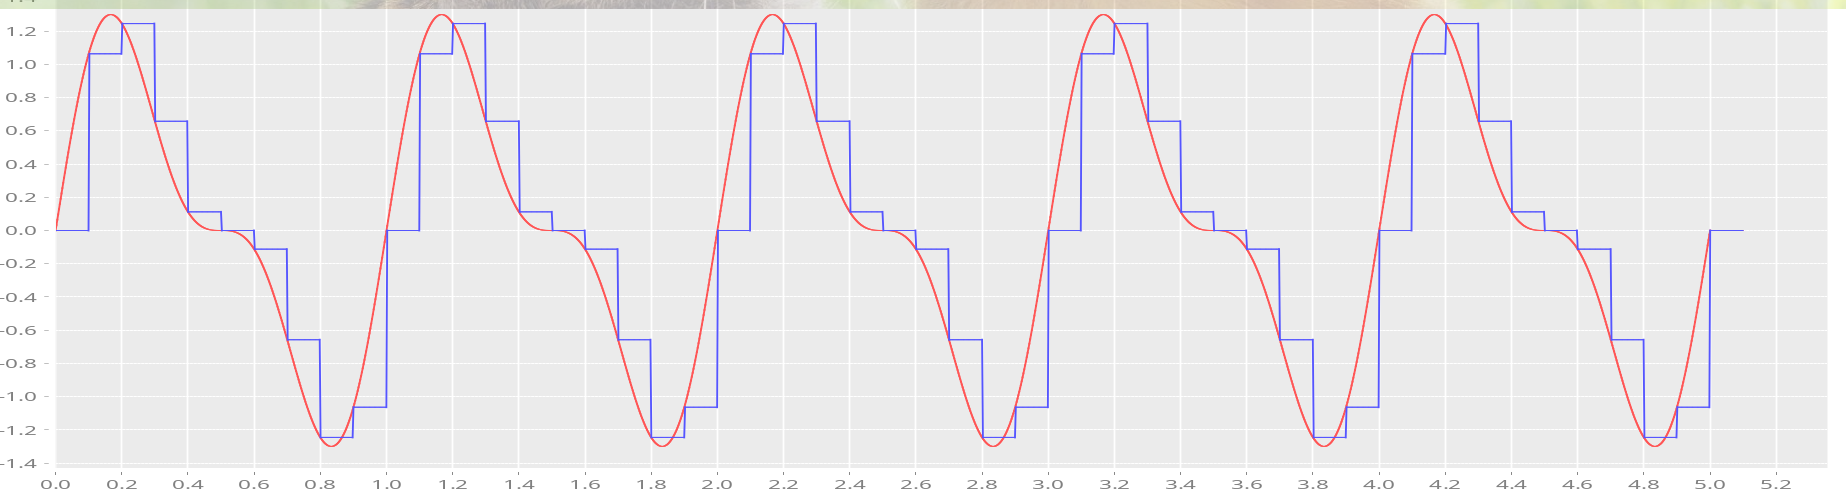
\includegraphics[width=\linewidth]{2z0.png}
	\caption{ekstrapolacja zerowego rzędu sygnału \ref{only}}
\end{figure}

\begin{figure}[H]
	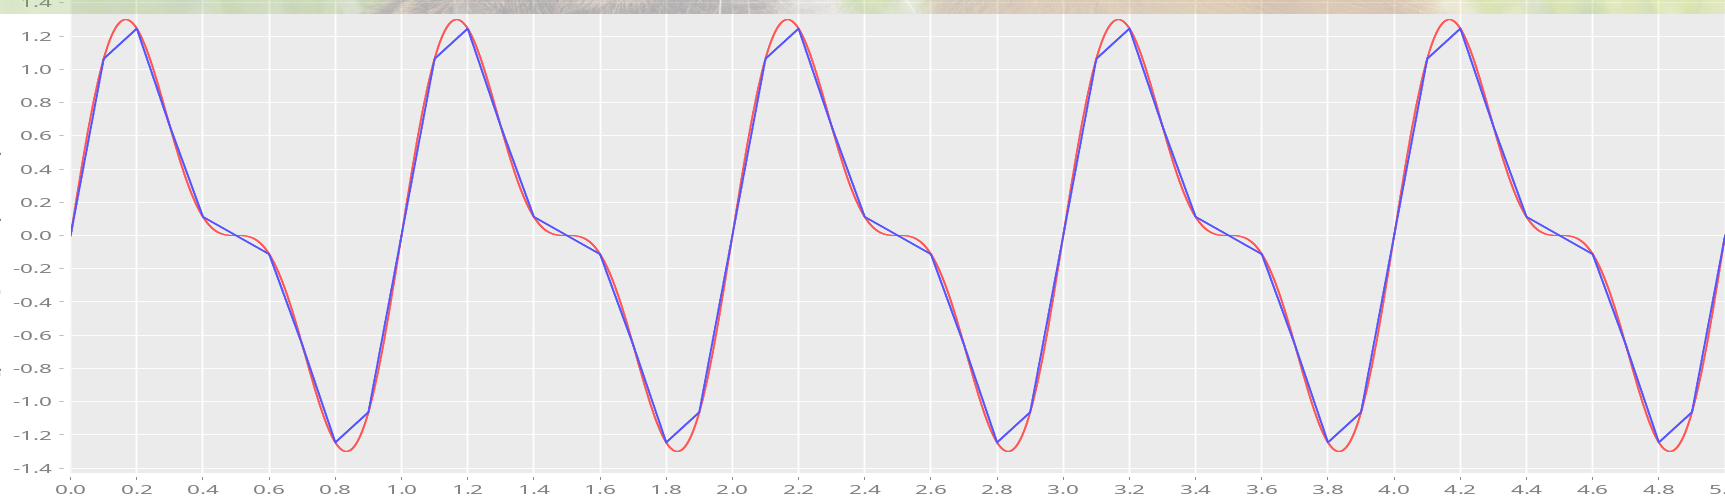
\includegraphics[width=\linewidth]{2z1.png}
	\caption{intprepolacja pierwszego rzędu sygnału \ref{only}}
\end{figure}

\begin{figure}[H]
	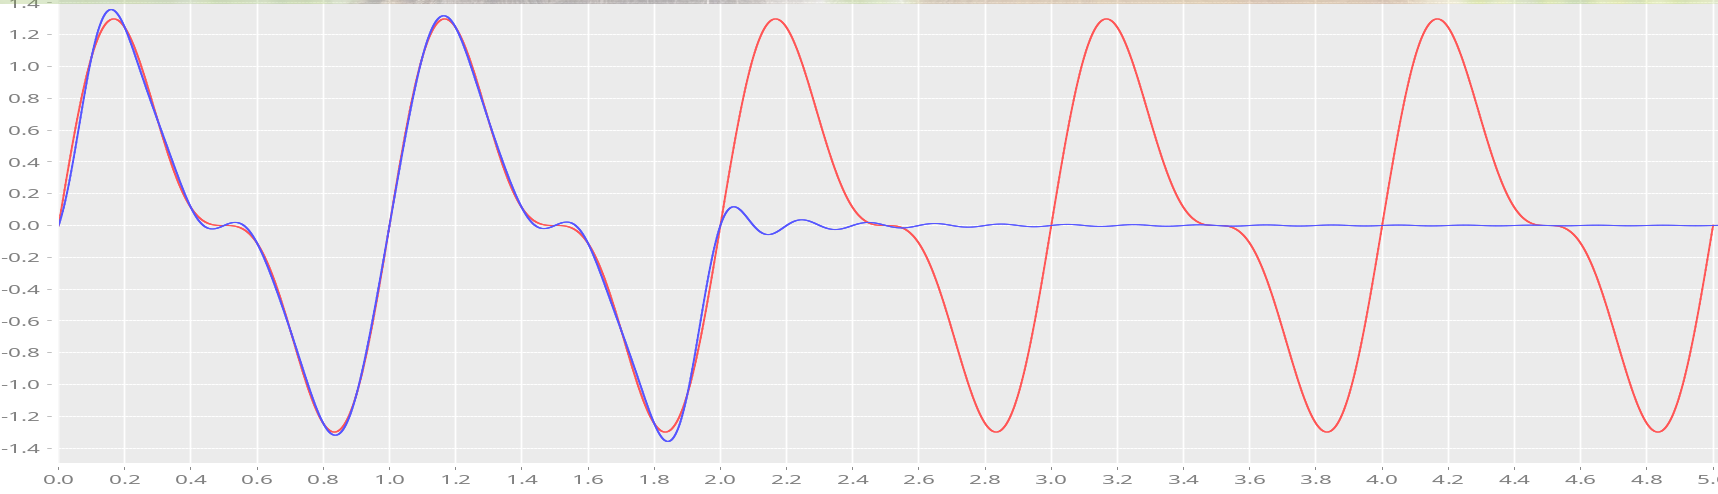
\includegraphics[width=\linewidth]{2zs20.png}
	\caption{intprepolacja funkcją sinc sygnału \ref{only} dla n=20}
\end{figure}

\begin{figure}[H]
	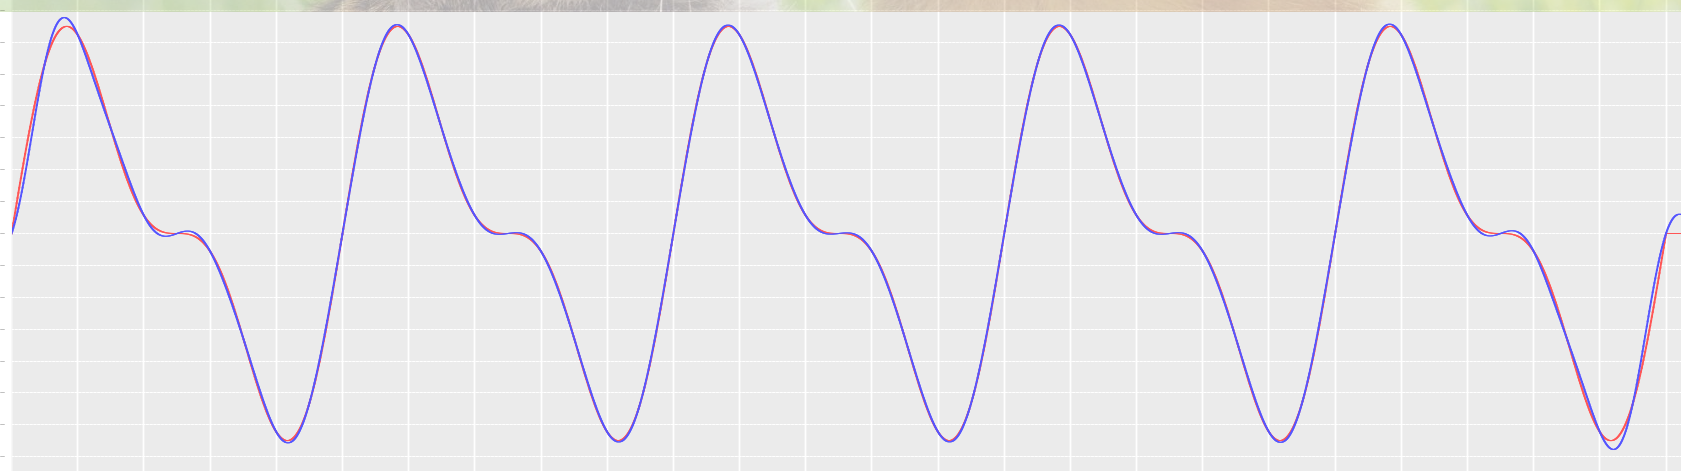
\includegraphics[width=\linewidth]{2zs80.png}
	\caption{intprepolacja funkcją sinc sygnału \ref{only} dla n=80}
\end{figure}

\begin{figure}[H]
	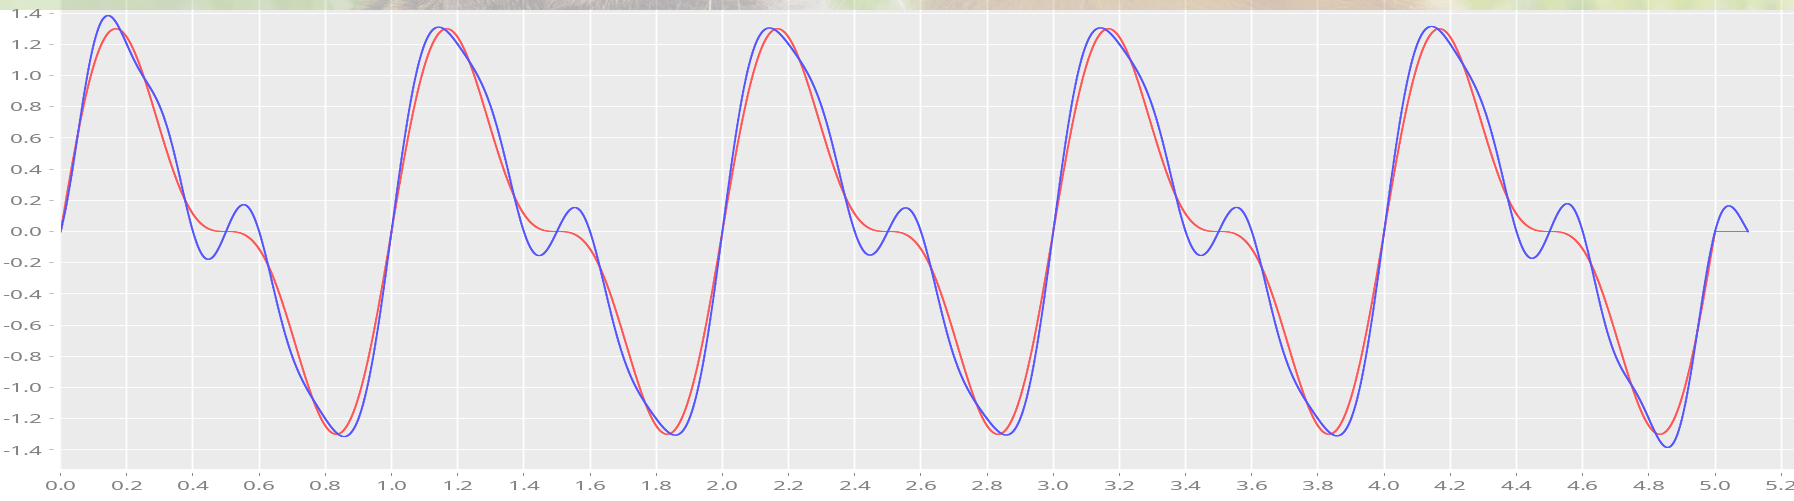
\includegraphics[width=\linewidth]{2zs80both.png}
	\caption{intprepolacja funkcją sinc sygnału \ref{both} dla n=80}
\end{figure}
%%%%%%%%%%%%%%%%%%%%%%%%%%%%%%%%%%%%%%%%%%%%%%%%%%%%%%%%%%%%%%%%%%%%%%%%%%%%%%%%%%%%%%%%%%%%%%%%%%%%%%%%%%%%%%%%%
% PODROZDZIA\xC5\x81 PT. ZALACZNIKI
%%%%%%%%%%%%%%%%%%%%%%%%%%%%%%%%%%%%%%%%%%%%%%%%%%%%%%%%%%%%%%%%%%%%%%%%%%%%%%%%%%%%%%%%%%%%%%%%%%%%%%%%%%%%%%%%%
%%%%%%%%%%%%%%%%%%%%%%%%%%%%%%%%%%%%%%%%%%%%%%%%%%%%%%%%%%%%%%%%%%%%%%%%%%%%%%%%%%%%%%%%%%%%%%%%%%%%%%%%%%%%%%%%%
% BIBLIOGRAFIA
%%%%%%%%%%%%%%%%%%%%%%%%%%%%%%%%%%%%%%%%%%%%%%%%%%%%%%%%%%%%%%%%%%%%%%%%%%%%%%%%%%%%%%%%%%%%%%%%%%%%%%%%%%%%%%%%%
\cite{instrukcja}
\renewcommand\refname{Bibliografia}
\bibliographystyle{plain}
\bibliography{ich}

\end{document}
